\section{Исследовательский раздел \hfill}
\vspace{\baselineskip}


\subsection{Технические характеристики}

Технические характеристики устройства, на котором выполнялись замеры времени:

\begin{itemize}[label=---]
	\item операционная система Windows 10;
	\item память 8 ГБ;
	\item процессор Intel® Core™ i5-6260U @ 1.80 ГГц, 2 физических ядра, 4 логических ядра.
\end{itemize}

Замеры времени выполнения реализаций алгоритмов проводились на ноутбуке, включенном в сеть электропитания. Во время тестирования ноутбук был нагружен только встроенными приложениями окружения, а также непосредственно разработанным приложением.

\subsection{Демонстрация работы программы}

На рисунке \ref{fig:example} представлен пример работы программы.
\clearpage

\begin{figure}[h!btp]
	\centering
	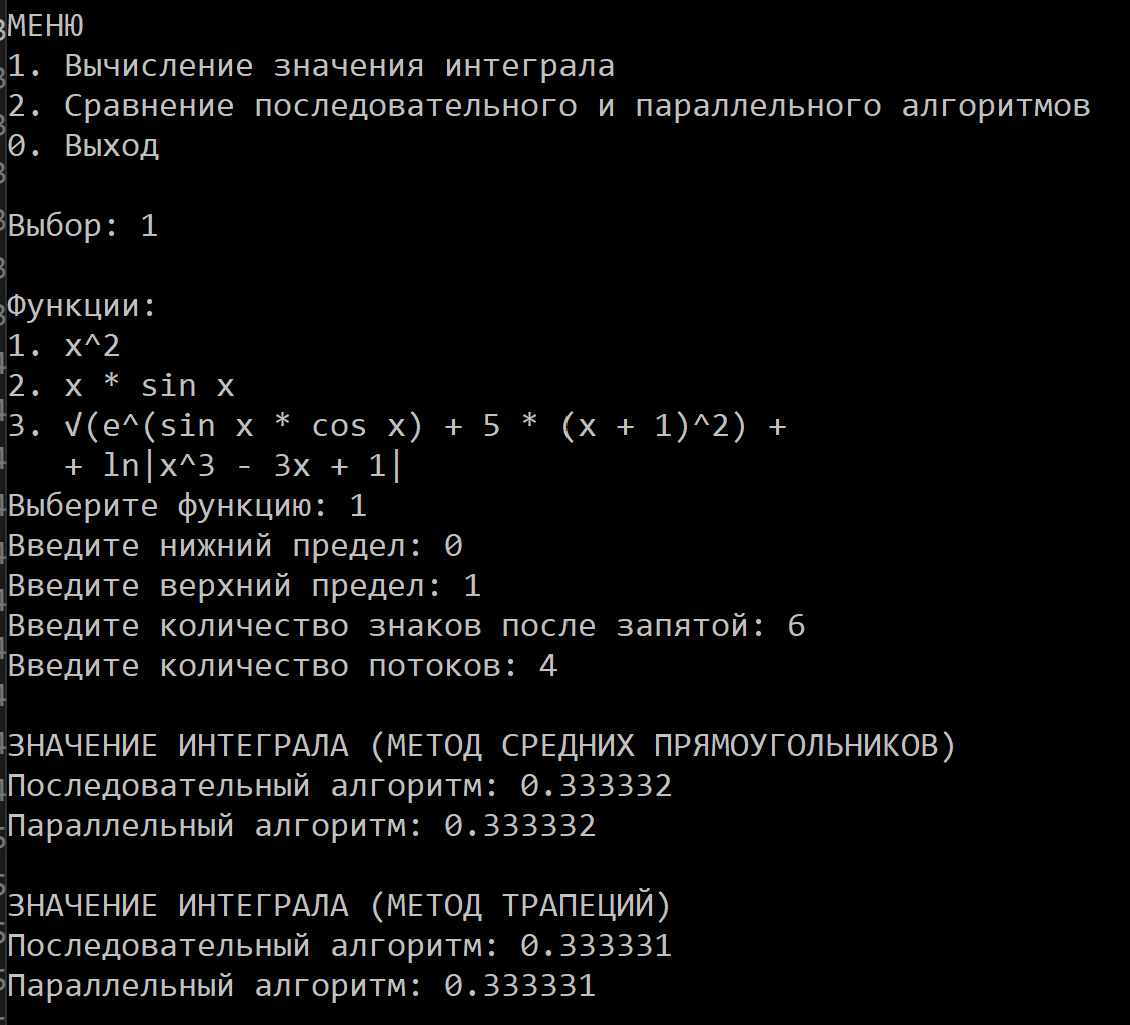
\includegraphics[width=280pt]{inc/example.png}
	\caption{Пример работы программы}
	\label{fig:example}	
\end{figure}

\subsection{Сравнение времени выполнения реализаций алгоритмов}

Для оценки времени работы последовательной и параллельной реализации алгоритма численного интегрирования был проведен эксперимент, в котором определялось влияние количества потоков и точности вычислений на время работы алгоритмов. Тестирование проводилось на количестве потоков, равном степеням 2 от 1 до 32, и на точности вычислений от 1 до 7 знаков после запятой. Так как от запуска к запуску время, затрачиваемое на выполнение алгоритма, менялось в определенном промежутке, необходимо было усреднить вычисляемые значения. Для этого каждый алгоритм в каждом случае запускался по 10 раз, и для полученных 10 значений определялось среднее арифметическое, которое заносилось в таблицу результатов.

В таблицах \ref{tab:threads-midpoint} и \ref{tab:threads-trapez} представлены результаты измерения времени работы параллельных реализаций алгоритмов в зависимости от числа потоков. На рисунках \ref{fig:gr1} и \ref{fig:gr3} представлены соответствующие графики. Для сравнения в таблицах и на графиках приведено также время последовательных реализаций.

В таблицах \ref{tab:eps-midpoint} и \ref{tab:eps-trapez} представлены результаты измерения времени работы последовательных и паралелльных реализаций алгоритмов в зависимости от числа знаков после запятой, соответствующие заданной точности вычислений интеграла. На рисунках \ref{fig:gr2} и \ref{fig:gr4} представлены соответствующие графики. Для наглядости на графике представлены только точки с точностью от 4 до 7 знаков после запятой.

\clearpage

\begin{table}[h]
    \begin{center}
    \begin{threeparttable}
        \captionsetup{justification=raggedright}
        \caption{\label{tab:threads-midpoint}Зависимость времени работы реализации от числа потоков (метод средних прямоугольников)}
        \begin{tabular}{|p{0.4\linewidth}|p{0.4\linewidth}|}
            \hline
            \bfseries Число потоков & \bfseries Время, нс \\
            \hline
            последовательный & 956216734 \\
            \hline
            1 & 949013547 \\
            \hline
            2 & 456833477 \\
            \hline
            4 & 404351737 \\
            \hline
            8 & 410132845 \\
            \hline
            16 & 428526431 \\
            \hline
            32 & 502791420 \\
            \hline
        \end{tabular}
    \end{threeparttable}
    \end{center}
\end{table} 

\begin{figure}[h!btp]
	\centering
	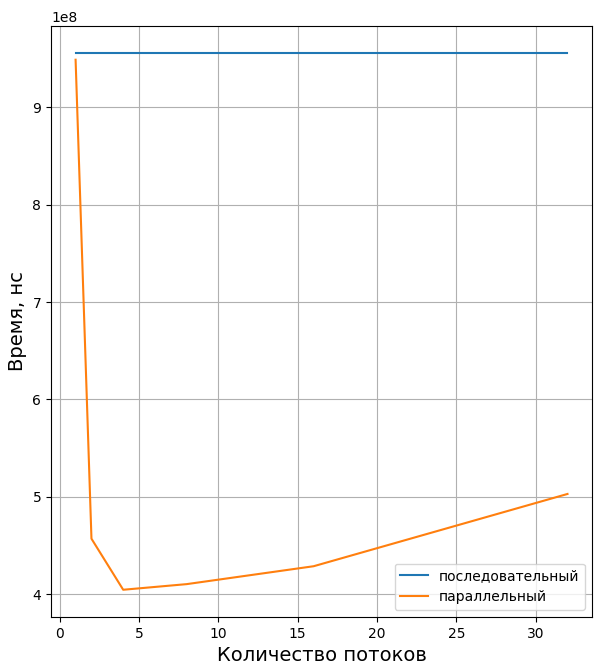
\includegraphics[width=300pt]{inc/gr1.png}
	\caption{Зависимость времени работы реализации от числа потоков (метод средних прямоугольников)}
	\label{fig:gr1}	
\end{figure}

\clearpage

\begin{table}[h]
    \begin{center}
    \begin{threeparttable}
        \captionsetup{justification=raggedright}
        \caption{\label{tab:eps-midpoint}Зависимость времени работы реализации от точности (метод средних прямоугольников)}
        \begin{tabular}{|p{0.2\linewidth}|p{0.25\linewidth}|p{0.35\linewidth}|}
            \hline
            \bfseries Точность & \bfseries 4 потока, нс & \bfseries Последовательный, нс \\
            \hline
            1e-1 & 10301220 & 527000 \\
            \hline
            1e-2 & 17464660 & 2857800 \\
            \hline
            1e-3 & 30899890 & 15451550 \\
            \hline
            1e-4 & 138586470 & 31622690 \\
            \hline
            1e-5 & 554727780 & 1561291940 \\
            \hline
            1e-6 & 1088159260 & 3061249760 \\
            \hline
            1e-7 & 1855569650 & 4569952270 \\
            \hline
        \end{tabular}
    \end{threeparttable}
    \end{center}
\end{table} 

\begin{figure}[h!btp]
	\centering
	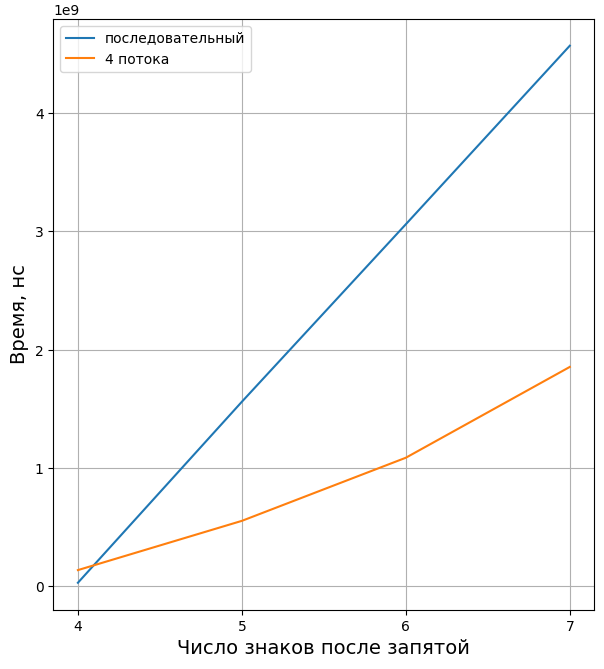
\includegraphics[width=300pt]{inc/gr2.png}
	\caption{Зависимость времени работы реализации от точности (метод средних прямоугольников)}
	\label{fig:gr2}	
\end{figure}

\clearpage

\begin{table}[h]
    \begin{center}
    \begin{threeparttable}
        \captionsetup{justification=raggedright}
        \caption{\label{tab:threads-trapez}Зависимость времени работы реализации от числа потоков (метод трапеций)}
        \begin{tabular}{|p{0.4\linewidth}|p{0.4\linewidth}|}
            \hline
            \bfseries Число потоков & \bfseries Время, нс \\
            \hline
            последовательный & 1234645093 \\
            \hline
            1 & 1224537253 \\
            \hline
            2 & 592657522 \\
            \hline
            4 & 404351737 \\
            \hline
            8 & 422857284 \\
            \hline
            16 & 465930467 \\
            \hline
            32 & 622873546 \\
            \hline
        \end{tabular}
    \end{threeparttable}
    \end{center}
\end{table} 

\begin{figure}[h!btp]
	\centering
	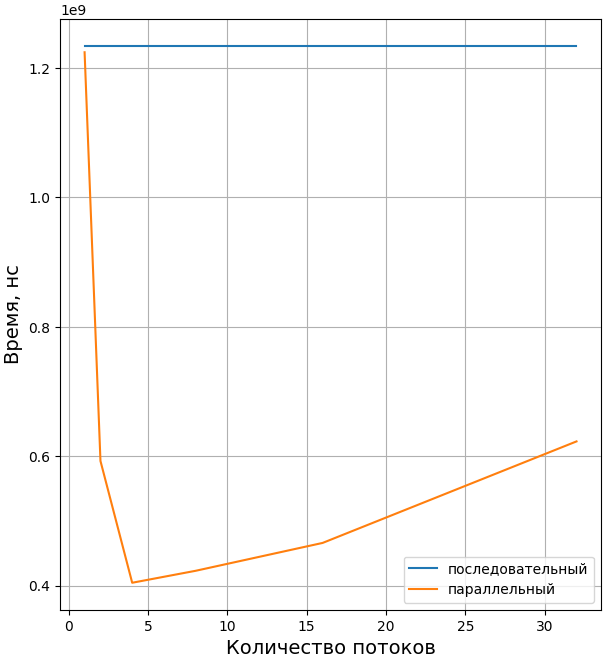
\includegraphics[width=300pt]{inc/gr3.png}
	\caption{Зависимость времени работы реализации от числа потоков (метод трапеций)}
	\label{fig:gr3}	
\end{figure}

\clearpage

\begin{table}[h]
    \begin{center}
    \begin{threeparttable}
        \captionsetup{justification=raggedright}
        \caption{\label{tab:eps-trapez}Зависимость времени работы реализации от точности (метод трапеций)}
        \begin{tabular}{|p{0.2\linewidth}|p{0.25\linewidth}|p{0.35\linewidth}|}
            \hline
            \bfseries Точность & \bfseries 4 потока, нс & \bfseries Последовательный, нс \\
            \hline
            1e-1 & 13298345 & 684562 \\
            \hline
            1e-2 & 22701673 & 3708234 \\
            \hline
            1e-3 & 39765463 & 20056836 \\
            \hline
            1e-4 & 179563421 & 40367467 \\
            \hline
            1e-5 & 721563426 & 2026647583 \\
            \hline
            1e-6 & 1613763452 & 3973745637 \\
            \hline
            1e-7 & 2412874563 & 5942874563 \\
            \hline
        \end{tabular}
    \end{threeparttable}
    \end{center}
\end{table} 

\begin{figure}[h!btp]
	\centering
	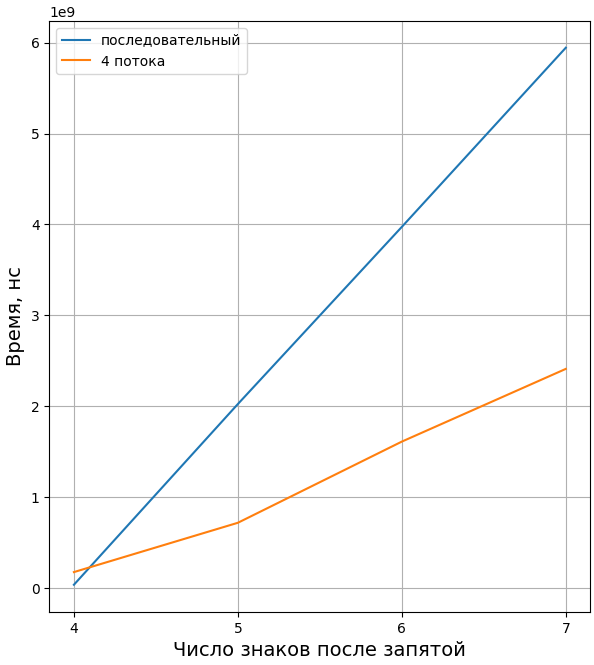
\includegraphics[width=300pt]{inc/gr4.png}
	\caption{Зависимость времени работы реализации от точности (метод трапеций)}
	\label{fig:gr4}	
\end{figure}

\clearpage

\subsection*{Вывод}
По результатам эксперимента можно сделать следующие выводы:
\begin{itemize}[label=---]
    \item по мере уменьшения числа потоков до числа логических ядер процессора время работы реализаций алгоритмов уменьшается;
    \item при превышении числа логических ядер время увеличивается, так как затрачивается время на переключение ядра между потоками;
    \item в зависимости от точности выигрыш от распараллеливания начинает проявляться только при точности от 5 знаков после запятой; это значит, что при меньшей точности время, затрачиваемое на создание и запуск потоков, больше чем выигрыш, получаемый от распараллеливания.
\end{itemize}

Таким образом, для достижения наибольшей скорости вычислений необходимо использовать число потоков, равное числу логических ядер процессора. При этом нецелесообразно использовать параллельную реализацию при проведении вычислений интегралов с точностью ниже, чем 5 знаков после запятой. 